\begin{tikzpicture}[scale=3.5]
  \begin{scope}[yshift=0\textwidth]
    \begin{scope}[xshift=0cm]
      \node [mybox] (box){
        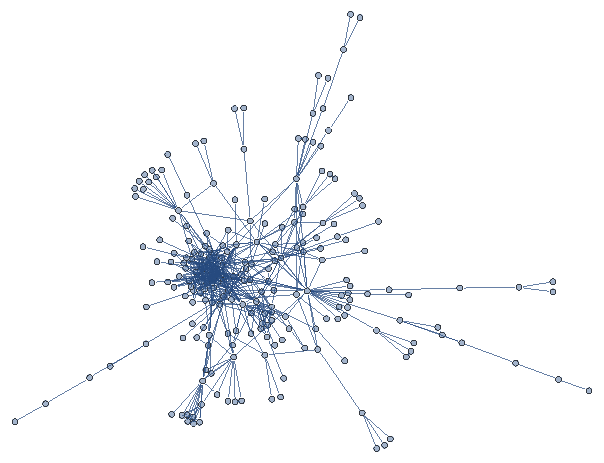
\includegraphics[width=0.45\textwidth]{../figures/graph_standard.pdf}
      };
    \end{scope}
    \begin{scope}[xshift=0.14\textwidth]
      \node [mybox] (box){
        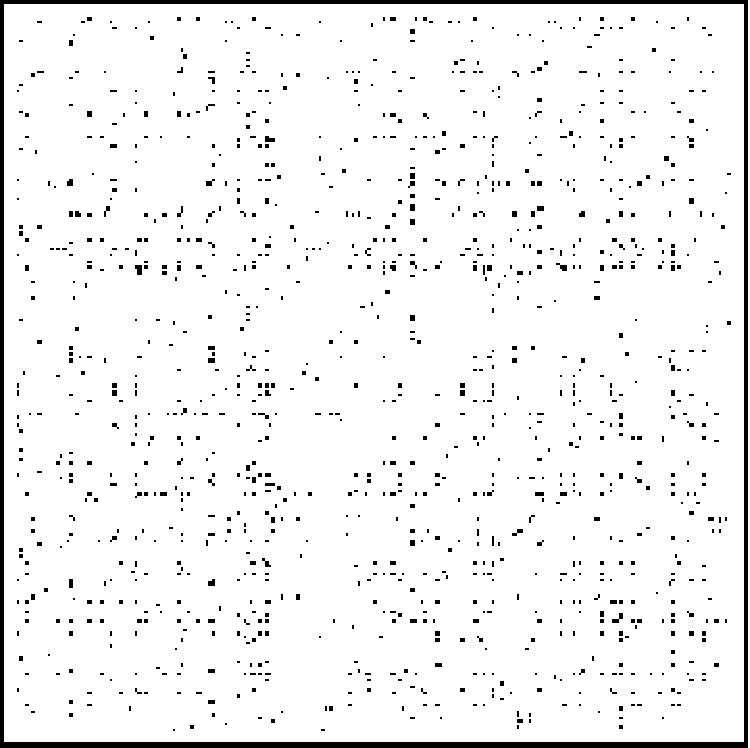
\includegraphics[width=0.36\textwidth]{../figures/unsorted_adjacency_matrix.pdf}
      };
    \end{scope}
  \end{scope}
%  \begin{scope}[yshift=-0.08\textwidth]
%    \begin{scope}[xshift=0cm]
%        \node[inner sep=0,text width=0.13\textwidth, text centered] (note1) at (0,0) {
%         \Large A protein interactome\ldots};
%     \end{scope}
%    \begin{scope}[xshift=0.14\textwidth]
%        \node[inner sep=0,text width=0.13\textwidth, text centered] (note1) at (0,0) {
%         \Large \ldots encoded as an array};
%     \end{scope}
%  \end{scope}
\end{tikzpicture}
